\documentclass{article}

\usepackage{subcaption}
\usepackage{amsmath}
\usepackage{color}
\usepackage{xcolor}
\usepackage{graphicx}
\usepackage{caption}
\usepackage{float}
\usepackage[bottom]{footmisc}
\usepackage[margin=.5in, tmargin=.5in]{geometry}
\setlength\parindent{0pt}
\captionsetup{justification=centering}

\title{Computer Science Large Practical Report}
\date{Tue, 20 Dec 2016}
\author{Traiko Dinev \textless s1448355\textgreater}

\begin{document}
	\maketitle

    \section{Aim}
		Aim
	
	\section{Simulator Architecture}
		The simulator has a decouple, observer pipeline, where everything is governed by an \textit{EventDispatcher} that schedules
		\textit{Events} and calls attached \textit{Observers}. The \textit{Areas}, the \textit{StatisticsAggregator} as well as the
		\textit{OutputFormatter} all have observers that listen to events happening. This way the output functionality and the statistics
		operate purely on the events happening and have no knowledge of the rest of the system, making them easier to develop and maintain.
		\\ \\
		See Figure~\ref{fig:fig1} for more details. The \textit{ExperimentManager} class creates one \textit{OutputFormatter}, \textit{StatisticsAggregator}
		and \textit{Simulation} and uses them for all runs necessary.

		\begin{figure}[H]
		\centering
			\includegraphics[width=.8\columnwidth]{resources/architecture.png}
			\captionof{figure}{Project Architecture \\\textit{file: resources/architecture.png}}
			\label{fig:fig1} 
		\end{figure}

	\subsection{Simulation Runs and Experiments}
		Each \textbf{run} of the program is governed by an \textit{ExperimentManager}, where actual experimentation behaves identically, while
		disabling detailed output (by not attaching an \textit{OutputFormmater} to the dispatcher.
		\\
		\\
		As such, each experiment contains a single \textit{Simulation}, which contains as many \textit{Area}s as necessary.
		Each \textit{Area} listens to events that happen in it and reacts accordingly. It also registers new disposal events and service events,
		as well as lorry events. Note the algorithm itself is separated and injected as a dependency in the constructor of the \textit{Area} class, thus
		separating that functionality out.


		\subsubsection{Pipeline}
		The input parser is the starting point of the application. Once we get a valid configuration file from the parser, we instantiate the
		\textit{ExperimentManager} class, which is in charge of creating each \textit{Simulation}, which create \textit{Areas}, which contain the actual
		simulation code. To glue things together, the \textit{EventDispatcher} is injected in the constructor of the Simulation, which in turn 
		injects it into each area class. Statistics and output are achieved similarly. The \textit{EventDispatcher} class is injected into an
		\textit{OutputFormatter} and into a \textit{StatisticsAggregator} class.
			\\
			\\
			See Figure~\ref{fig:fig2} for a sequence diagram illustrating the start of the simulation and a cycle of events.

		\begin{figure}[H]
		\centering
			\includegraphics[width=1\columnwidth]{resources/start_sequence.png}
			\captionof{figure}{Startup Sequence \\\textit{file: resources/start\_sequence.png}}
			\label{fig:fig2} 
		\end{figure}

	\subsection{Route Planning}
	Route planning is done separately in the \textbf{DijkstraRoutePlanner} class. The route planner uses Dijkstra's algorithm each time
	a route is needed and two different heuristics for selecting the next bin to be serviced. The \textit{greedy} algorithm always services
	bins according to their occupancy (or volume). The \textit{priority} algorithm always services the closest bin. Both always use only the bins
	that need servicing (i.e. they do not ever calculate a path that would empty a bin that has not exceeded the occupancy threshold).

	\subsection{Optimization}
		The greedy algorithm is generally faster than the priority algorithm and hence the default setting of the algorithm it \textit{dynamic}, which
		selects one of the two versions based on how many bins are to be serviced. The algorithm also uses caching to save already calculated paths
		so that they are not computed twice. The cache has a limit (TODO) and all of the above settings can be overridden via command-line parameters.
		
	\subsubsection{Caching}
		See figure~\ref{fig:fig3} for effects of caching on the performance of the algorithm. All tests were done on a small area (5x5), a medium sized area (50x50)
		and a big area (300x300). All areas run for 100 hours and are otherwise a derivation of the \textit{basic\_input}. The simulator was run with the \textit{-d -b} options
		to produce timing details and disable output. For any test, we take the average of 10 results, since the simulation is stochastic. Outliers were not removed
		in this scenario.

		\begin{figure}[H]
		\centering
			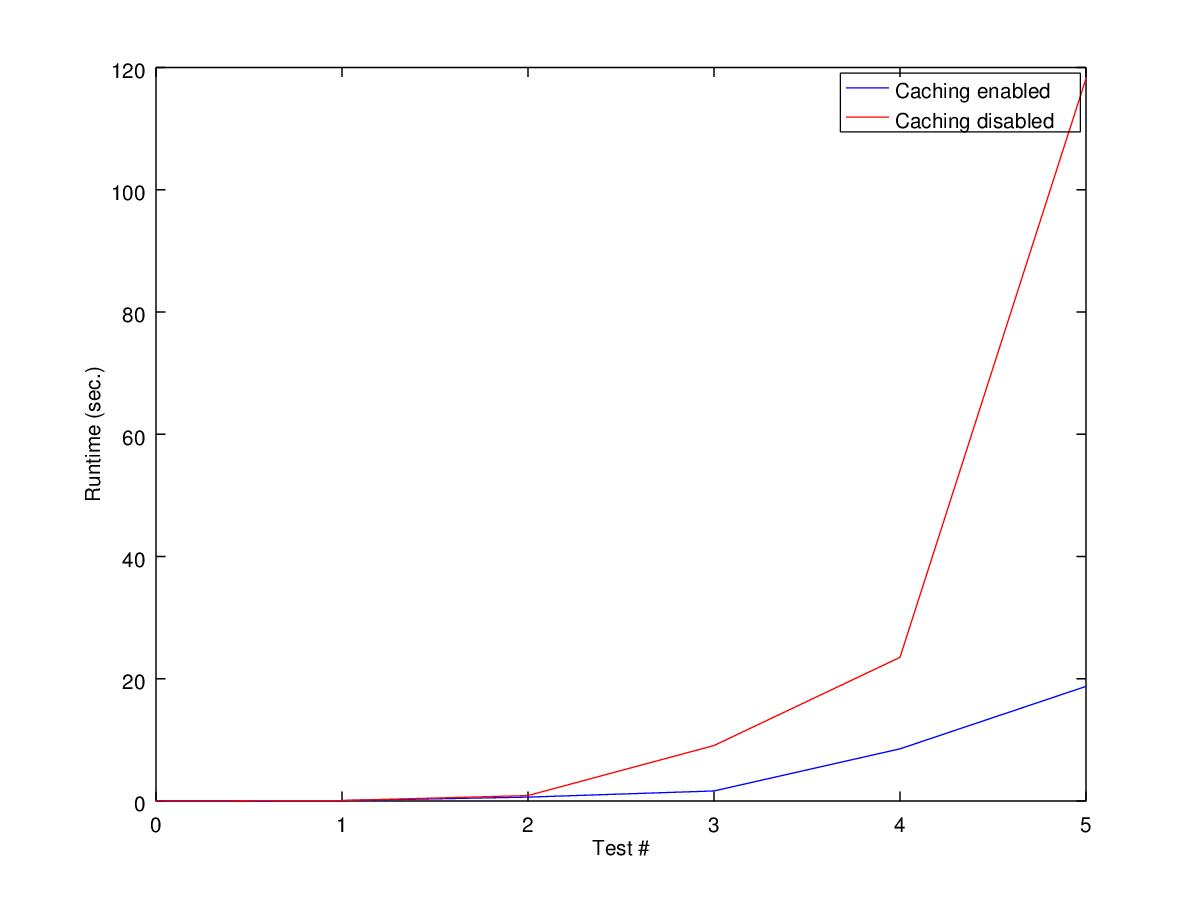
\includegraphics[width=.55\columnwidth]{resources/caching_performance.jpg}
			\captionof{figure}{Performance with/without caching \\\textit{file: resources/caching\_performance.jpg}}
			\label{fig:fig3}
		\end{figure}

		\subsubsection{Cache size}
			Caching size also makes a significant different, but only up to the number of possible paths. We do not let variable cache sizes,
			since that is too hard to benchmark. Instead, we cap the cache size at $100,000$. This accomodates for a total number of $\frac{ceil(sqrt(100000))}{2} = 159$ vertices
			all connected to each other (all possible paths). However, a map of 159x159, which has every vertex connected to every other is \textbf{very} unlikely. Below in Figure ~\ref{fig:fig4}
			you can see the effect of cache size on a map of 300x300 with several experiments, average of 3 results taken for each cache size.
		
			\begin{figure}[H]
			\centering
				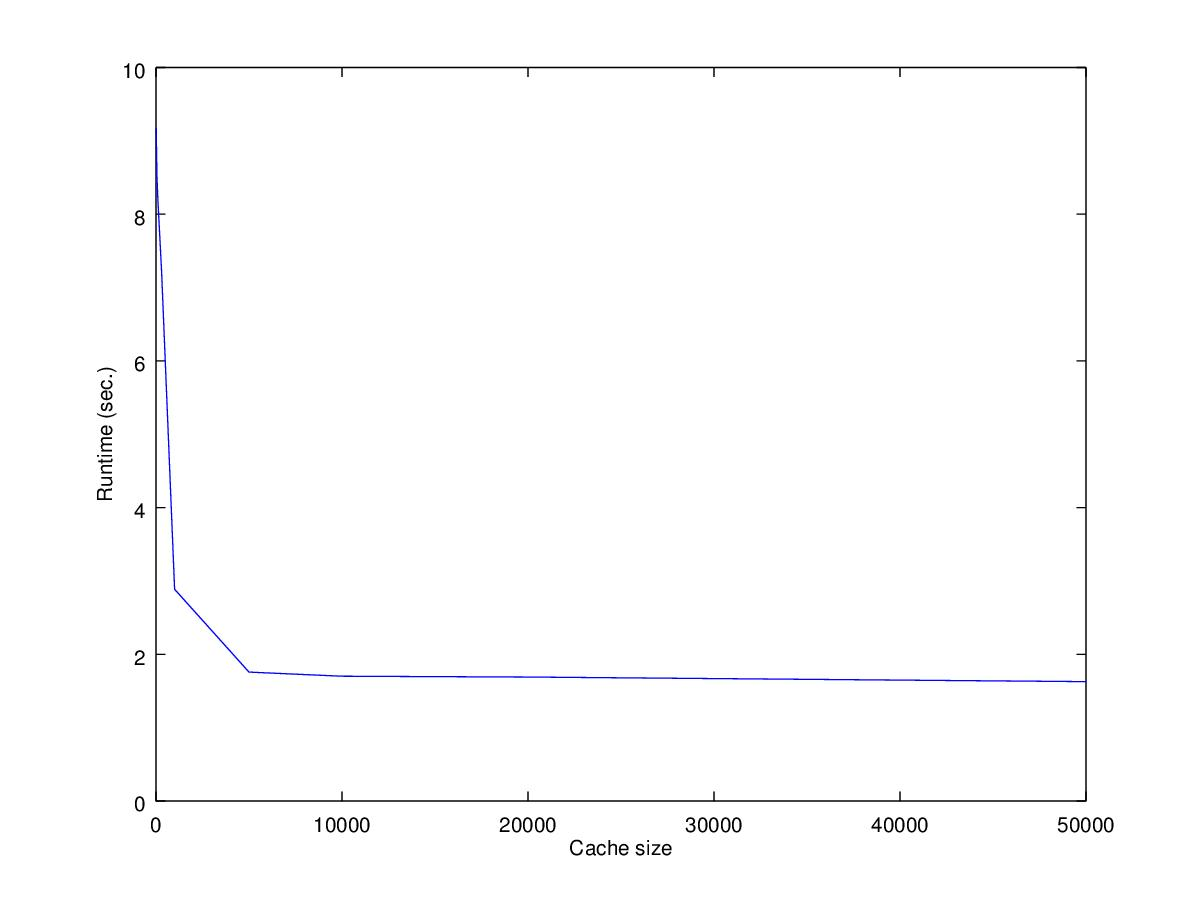
\includegraphics[width=.55\columnwidth]{resources/cache_size.jpg}
				\captionof{figure}{Effects of cache size on performance \\\textit{file: resources/cache\_size.jpg}}
				\label{fig:fig4}
			\end{figure}
			

	\section{Simulation Results}

		\subsection{Test inputs}
			To evaluate the simulation, two distinct input files were used. They model two different realistic scenarious.
			The first one (\textit{Three Neighborhoods}) \footnote{File: test/inputs/statistics\_collection/three\_neighborhoods.txt} models three separate connected neighborhoods, where the paths
			within the neighborhoods are shorter than the path between them. (See figure~\ref{fig:fig5a}) 
			\\
			\\
			The second input (\textit{Big Cluster}) \footnote{File: test/inputs/statistics\_collection/big\_cluster.txt} models one big area where all of the bins are interconnected and paths
			within it are comparable in distance/duration. (See figure~\ref{fig:fig5b})
			\\
			\\
			We expect the priority algorithm, which selects bins based on their distance from the current location, to work
			better on the \textit{Three neighborhoods} area and for them to work comparably well on the big cluster area.

			\begin{figure}[H]
				\centering
				\begin{subfigure}[b]{.5\textwidth}
					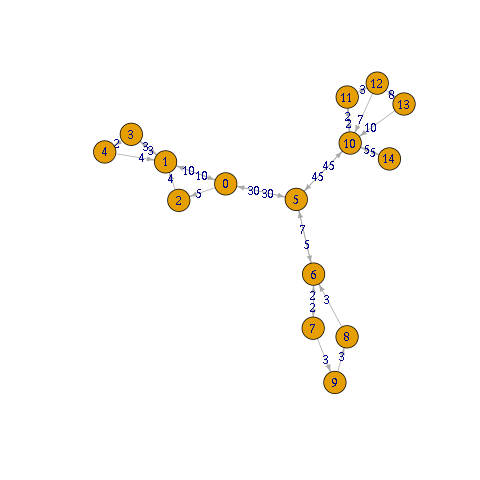
\includegraphics[width=\textwidth]{resources/three_neighborhoods.png}
					\caption{Three Neighborhoods \\\textit{file: resources/three\_neighborhoods.png}}
					\label{fig:fig5a}
				\end{subfigure}\hfill%
				\begin{subfigure}[b]{.5\textwidth}
					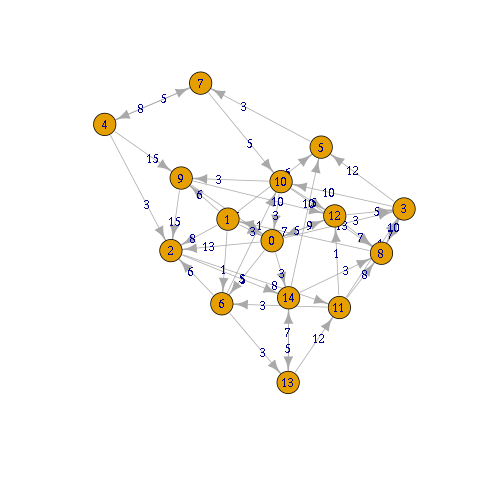
\includegraphics[width=\textwidth]{resources/big_cluster.png}
					\caption{Big Cluster \\\textit{file: resources/three\_neighborhoods.png}}
					\label{fig:fig5b}
				\end{subfigure}
				\label{fig:fig5}
				\caption{Areas used for evaluation}
			\end{figure}

		\subsection{Bin Occupancy Evolution}
		The first metric of interest is the bin volume plotted against time. In figure~\ref{fig:fig6a} and figure~\ref{fig:fig6b} we
		can see the average volume of the bins for the \textit{Three Neighborhoods} and \textit{Big Cluster} areas. In both
		$disposalDistrShape\ =\ 3$ (3 bags per hour) and $serviceFreq = 0.04167$ (one service daily), but in ~\ref{fig:fig6a}
		$disposalDistrRate\ = \ 5.0$, while in ~\ref{fig:fig6b} $disposalDistrRate\ =\ 3$. Both of the simulations stop after
		a week with a warm-up time of a day and both have a bag volume of $0.05$ with a maximum bin volume of $2$.
		\\
		\\
		Since the mean of the Erlang-K distribution is $\mu\ =\ \frac{k}{\lambda}$, in each case we would expect the average bin content
		before each service period to follow:
    	\begin{equation}
			bin\_content\ =\ \frac{time\_between\_service\_periods}{\mu_{erlang}}\ *\ bin\_volume
		\end{equation}
		\\
		\\
		Given that all bins are independent\footnote{By the specifications}. This yields $1.8\ m^3$ average volume for \textit{Three Neighborhoods}
		and $3\ m^3$ for \textit{Big Cluster}, which is what is observed in the graphs. Note, however, that the bins cannot have a maximum volume of
		$2\ m^3$, therefore on the second graph we see the "cap".


		\begin{figure}[H]
			\centering
			\begin{subfigure}[b]{.5\columnwidth}
				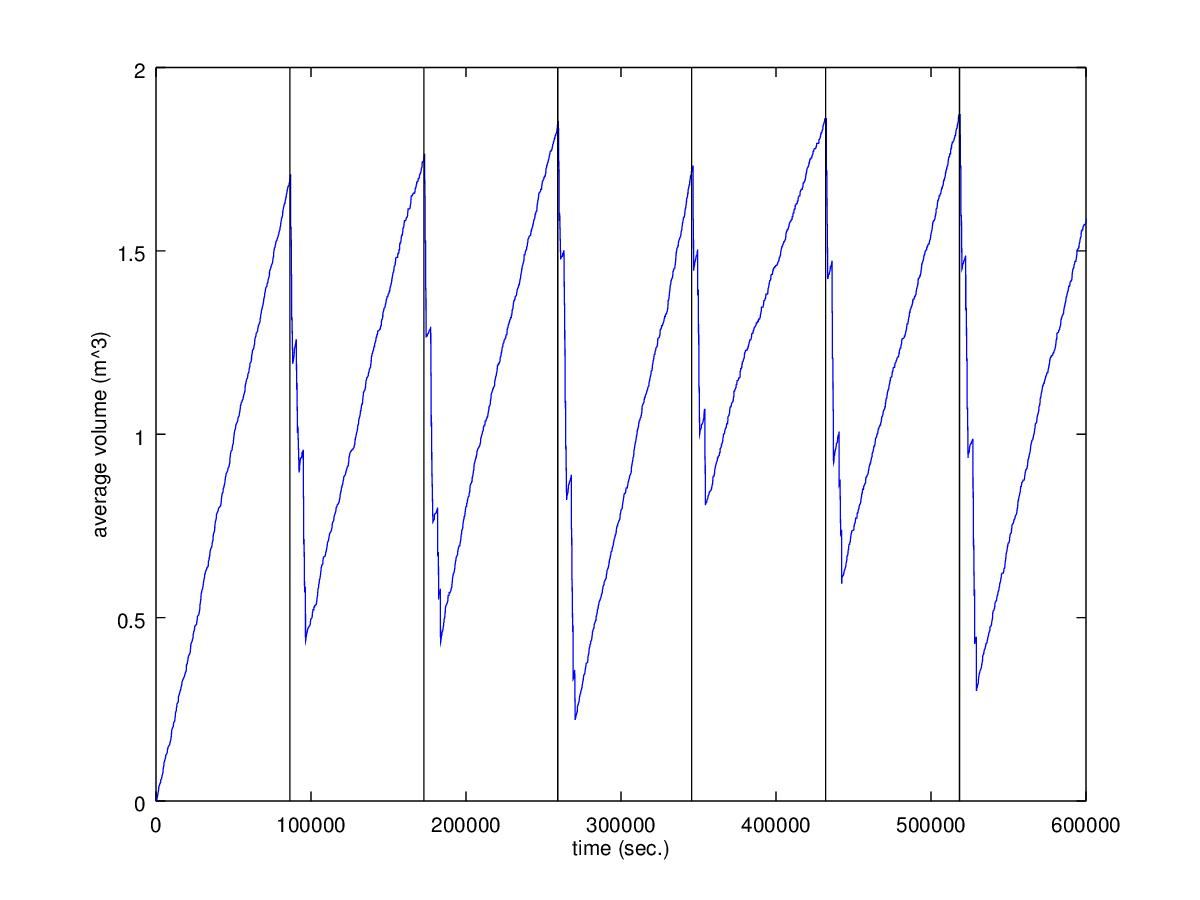
\includegraphics[width=\textwidth]{resources/occupancy_three_neighborhoods.jpg}
				\caption{Bin Volume Evolution (Three Neighborhoods) \\\textit{file: resources/occupancy\_three\_neighborhoods.png}}
				\label{fig:fig6a}
			\end{subfigure}\hfill%
			\begin{subfigure}[b]{.5\columnwidth}
				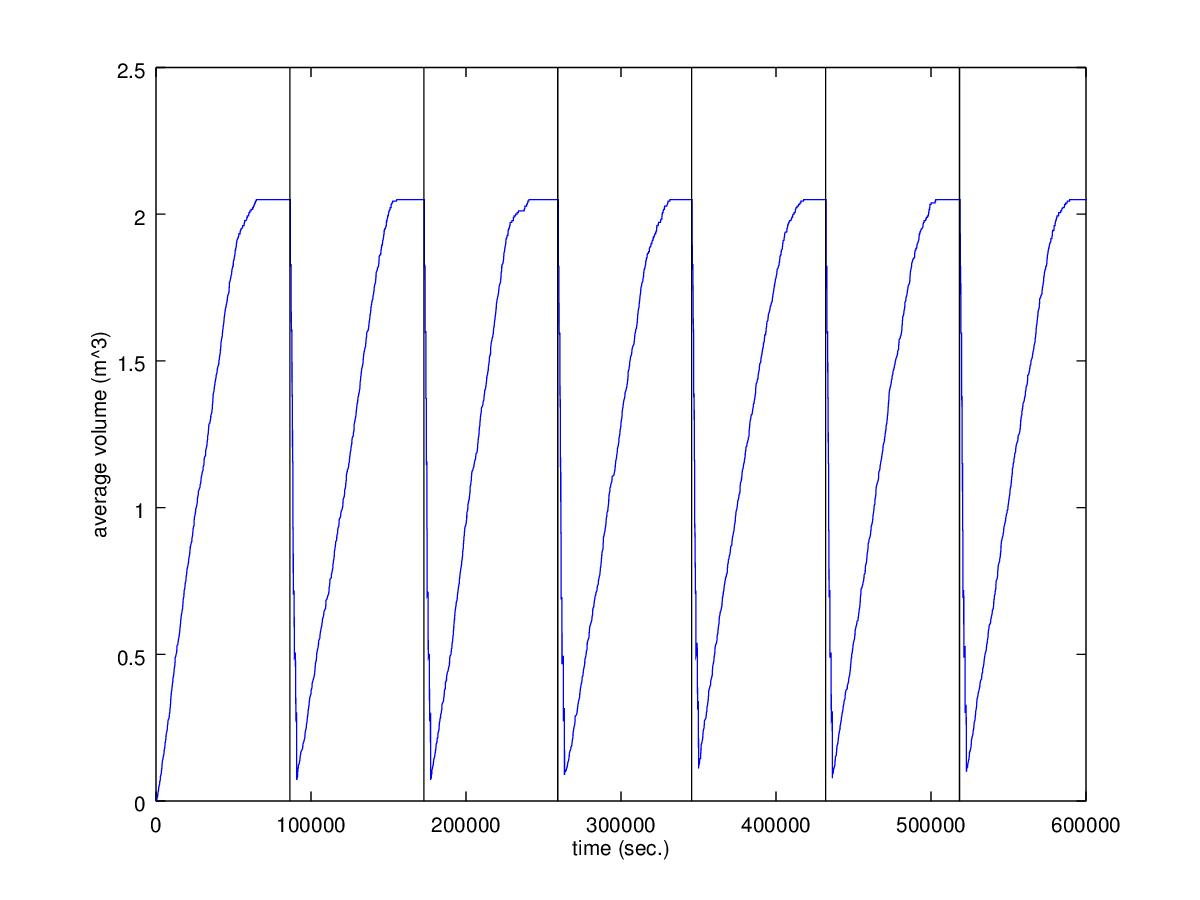
\includegraphics[width=\textwidth]{resources/occupancy_big_cluster.jpg}
				\caption{Bin Volume Evolution (Big Cluster) \\\textit{file: resources/occupancy\_big\_cluster.png}}
				\label{fig:fig6b}
			\end{subfigure}
			\label{fig:fig6}
		\end{figure}



			

\end{document}
